\chapter{Construção da Aplicação}\label{chp:des}

\section{Estudo de caso: principais assuntos e abordagens}

\subsection{Matrizes curriculares}

A análise das matrizes curriculares do Ensino Fundamental I, especificamente para o 4º ano na disciplina de Matemática, é fundamental para identificar os conteúdos essenciais e as lacunas existentes no ensino atual. Este estudo comparativo entre o conteúdo programático do Colégio Salesiano do Salvador e o Referencial Curricular Municipal de Salvador, conforme apresentado posteriormente no capitulo de resultados, permitiu compreender as diferenças significativas em suas abordagens e detalhamentos.

Enquanto o Colégio Salesiano adota uma estrutura mais detalhada e segmentada por trimestres, o Referencial Municipal apresenta uma abordagem integrada e contínua. Segundo \cite{mesquita2023gamificacao}, a falta de uniformidade nos conteúdos pode dificultar a consolidação do aprendizado, evidenciando a necessidade de ferramentas que alinhem essas discrepâncias e ofereçam uma educação matemática mais consistente.

\subsection{Comparação e extração de assuntos em comum}

A comparação entre as matrizes curriculares permitiu extrair oito unidades temáticas principais que são comuns e essenciais para o ensino de matemática no 4º ano: operações básicas (adição, subtração, multiplicação e divisão), frações, álgebra, geometria, grandezas e medidas, probabilidade e estatística, educação financeira e algarismos romanos. Detalhes sobre essas unidades podem ser encontrados em \textit{capitulos/4\_Contrução da Aplicação.tex}.

Essa extração foi fundamental para garantir que o aplicativo aborde os conteúdos mais relevantes e que estejam em consonância com as expectativas educacionais, proporcionando uma base sólida para os alunos avançarem em tópicos mais complexos no futuro.

\subsection{Classificação por grau de relevância}

Os conteúdos selecionados foram classificados com base em sua relevância para o desenvolvimento das competências matemáticas dos alunos. Priorizaram-se temas fundamentais, como as operações básicas e a resolução de problemas, essenciais para o entendimento de conceitos matemáticos mais avançados.

Conforme evidenciado por \cite{mesquita2023gamificacao}, essa classificação permite uma progressão natural do aprendizado, facilitando a assimilação dos conteúdos e mantendo o aluno motivado através de desafios adequados ao seu nível de conhecimento.

\subsection{Validação com professores do ensino fundamental I}

A validação dos conteúdos e abordagens propostas foi realizada com a participação ativa de professores do Ensino Fundamental I. Como documentado em nos resultados, foram aplicados questionários e realizadas entrevistas para avaliar aspectos como usabilidade do aplicativo, eficácia pedagógica e potencial de engajamento dos alunos.

Essa etapa foi crucial para refinar o aplicativo, garantindo que ele atenda às necessidades reais do ambiente escolar e esteja alinhado com as práticas pedagógicas atuais. A colaboração com os educadores não apenas fortaleceu a relevância do estudo, mas também destacou a contribuição original deste trabalho ao integrar teoria e prática na elaboração de uma solução inovadora para o ensino da matemática básica.

\begin{longtable}{|m{1.5cm}|m{3.5cm}|m{4.5cm}|m{5cm}|}
\hline
\textbf{Unidade} & \textbf{Tópico} & \textbf{Sobre esta unidade} & \textbf{Sugestões} \\
\hline
\endfirsthead

\hline
\textbf{Unidade} & \textbf{Tópico} & \textbf{Sobre esta unidade} & \textbf{Sugestões} \\
\hline
\endhead

\hline
\endfoot

\hline
\endlastfoot

I & Números: soma e subtração & Nessa unidade temática vamos estudar noções básicas de adição e subtração. & 
Antes iniciar as operações (adição, subtração, multiplicação, divisão) seria interessante trazer o sistema de numeração decimal: leitura, escrita, comparação e ordenação de números naturais de até cinco ordens. Usar o termo adição ao invés de soma. Depois de abordar essas duas operações separadamente vale relacionar as duas: adição e subtração. \\
\hline
II & Números: multiplicação e divisão & Nessa unidade temática vamos estudar noções de multiplicação e divisão. & 
Depois de abordar essas duas operações separadamente vale relacionar as duas: multiplicação e divisão. \\
\hline
III & Números: frações & Nessa unidade temática vamos estudar frações. & 
Trazer já aqui a representação decimal escrevendo valores do sistema monetário brasileiro. Isso ajudará na Unidade VIII de Educação Financeira. \\
\hline
IV & Álgebra & Nessa unidade temática vamos estudar padrões numéricos e determinar valores faltantes. & 
Usar o termo sequências numéricas ao invés de padrões numéricos. \\
\hline
V & Geometria & Nessa unidade temática vamos estudar paralelismo, área de superfícies, ângulos e algumas formas geométricas básicas. & 
Antes de paralelismo ajudaria iniciar reforçando conceitos como localização e movimentação: pontos de referência, direção e sentido. Depois das formas geométricas poderiam finalizar acrescentando os sólidos geométricos básicos conectando com suas planificações. \\
\hline
VI & Grandezas e medidas & Nessa unidade temática vamos estudar as principais unidades de medida. & 
Se possível trazer as 5 unidades de medida: comprimento, massa, capacidade, tempo e temperatura. \\
\hline
VII & Probabilidade e estatística & Nessa unidade temática vamos estudar gráficos e eventos aleatórios. & 
Antes de iniciar probabilidade trazer problemas de contagem simples que possam resolver por agrupamentos e escrita multiplicativa. \\
\hline
VIII & Educação financeira & Nessa unidade temática vamos estudar um pouco sobre educação financeira. & 
Trazer problemas utilizando o sistema monetário brasileiro. \\
\hline
IX (Bônus) & Algarismos romanos & Nessa unidade temática vamos aprender a ler algarismos romanos. & 
Achei ótimo esse bônus se possível acrescentar antes o sistema de numeração egípcio depois segue com o sistema de numeração romano. \\

\caption{Feedbacks e observações sobre o conteúdo e sua abordagem}




\end{longtable}

\textbf{Matriz de assuntos que irão ser abordados na aplicação após o estudo de casos}


\section{Comparativo de aplicações de ensino}

\textbf{Aplicação Duolingo}

Duolingo é uma plataforma de aprendizado de idiomas amplamente popular, acessível via website e aplicativos móveis. Fundada com o objetivo de tornar o aprendizado de idiomas acessível e divertido, a plataforma oferece uma maneira inovadora e gamificada de aprender novas línguas. 

\begin{enumerate}
    \item \textbf{Como Funciona}
    
    A metodologia do Duolingo baseia-se em atividades interativas e lições curtas que incentivam a prática diária. As lições são estruturadas em níveis e unidades, cobrindo aspectos como vocabulário, gramática, leitura, escrita e pronúncia. A gamificação é um componente crucial, com elementos como pontos, conquistas e um sistema de vidas que motiva os usuários a continuar aprendendo.

    \item \textbf{Tecnologias Inovadoras}

    O Duolingo se destaca por sua aplicação inovadora de tecnologias para aprimorar a experiência de aprendizado de idiomas:

    \begin{itemize}
        \item \textbf{Aprendizado de Máquina e Inteligência Artificial (IA):}
        \begin{itemize}
            \item \textbf{Algoritmos Adaptativos:} Personalizam o conteúdo e as atividades de acordo com o ritmo e estilo de aprendizado de cada usuário, otimizando a eficácia do ensino.
            \item \textbf{Avaliação Automática:} Oferece feedback instantâneo sobre a pronúncia e escrita, auxiliando na correção de erros e no aprimoramento contínuo.
            \item \textbf{Chatbots e Assistentes Virtuais:} Permitem a prática da conversação de forma interativa e personalizada, simulando situações reais de comunicação.
        \end{itemize}
        
        \item \textbf{Processamento de Linguagem Natural (PLN):}
        \begin{itemize}
            \item \textbf{Compreensão e Geração de Texto:} Possibilita a criação de exercícios e atividades que simulam a comunicação natural, como diálogos e textos escritos.
            \item \textbf{Análise Semântica:} Garante a precisão e relevância das traduções e do conteúdo apresentado aos usuários.
            \item \textbf{Reconhecimento de Fala:} Permite a avaliação da pronúncia e entonação do usuário, aprimorando suas habilidades orais.
        \end{itemize}

        \item \textbf{Gamificação:}
        \begin{itemize}
            \item \textbf{Sistemas de Pontos e Recompensas:} Motivam os usuários a continuar aprendendo e progredindo na plataforma.
            \item \textbf{Níveis e Desafios:} Criam um senso de conquista e engajamento, mantendo o interesse dos usuários.
            \item \textbf{Tabelas de Classificação e Competição Amistosa:} Estimulam a interação entre os usuários e promovem a colaboração.
        \end{itemize}
    \end{itemize}

    \item \textbf{UX/UI: Uma Experiência de Aprendizagem Intuitiva e Agradável}
    
    O Duolingo se preocupa em oferecer uma interface amigável e intuitiva que facilite o aprendizado:

    \begin{itemize}
        \item \textbf{Design Simples e Minimalista:} Prioriza a clareza e a organização da informação, evitando distrações e facilitando a navegação.
        \item \textbf{Recursos Visuais Atraentes:} Utiliza cores vibrantes, ilustrações e animações para tornar o aprendizado mais engajador e divertido.
        \item \textbf{Acessibilidade Universal:} Garante que a plataforma possa ser utilizada por pessoas com diferentes habilidades e necessidades, incluindo deficientes visuais e auditivos.
        \item \textbf{Experiência Personalizada:} Permite que os usuários personalizem a interface de acordo com suas preferências, como idioma base e ritmo de aprendizado.
    \end{itemize}

    \item \textbf{Idiomas Oferecidos}
    
    Duolingo oferece uma ampla gama de cursos de idiomas, desde os mais comuns, como inglês, espanhol e francês, até idiomas menos comuns, como esperanto, gaélico escocês e navajo. A diversidade de opções permite que usuários de diferentes interesses e necessidades encontrem cursos que atendam às suas expectativas.

    \item \textbf{Recursos e Funcionalidades}
    
    Além das lições padrão, Duolingo Plus é a versão premium que remove anúncios e oferece outras vantagens. A plataforma também disponibiliza podcasts em idiomas como inglês e espanhol, histórias interativas que ajudam na compreensão de leitura e eventos ao vivo onde os usuários podem praticar conversação.

    \item \textbf{Vantagens e Desvantagens}
    
    \begin{itemize}
        \item \textbf{Vantagens:}
        \begin{itemize}
            \item Acessibilidade gratuita
            \item Metodologia gamificada e divertida
            \item Diversidade de idiomas
        \end{itemize}

        \item \textbf{Desvantagens:}
        \begin{itemize}
            \item Limitações na profundidade do conteúdo
            \item Dependência de conexão com a internet para algumas funcionalidades
            \item Críticas sobre a eficácia do aprendizado para níveis avançados
        \end{itemize}
    \end{itemize}

    \item \textbf{Impacto e Estatísticas}
    
    Duolingo tem um impacto global significativo, com mais de 500 milhões de downloads e uma base de usuários ativa mensal de aproximadamente 40 milhões. A plataforma também é usada por escolas e educadores para complementar o ensino de idiomas.

    \item \textbf{Futuro e Inovações}
    
    O Duolingo continua a inovar, incorporando inteligência artificial para personalizar a experiência de aprendizado e desenvolver novos recursos. A empresa planeja expandir seu alcance e melhorar a eficácia dos cursos, explorando novas tecnologias e métodos pedagógicos.
    \footnote{\url{https://play.google.com/store/apps/details?id=com.duolingo&hl=pt_BR}}
\end{enumerate}
   


    


    \begin{itemize}
    \item \textbf{Khan Academy}

    A Khan Academy se destaca como uma plataforma educacional online que democratiza o acesso ao conhecimento, oferecendo uma vasta gama de cursos gratuitos em diversas disciplinas. Fundada com a missão de prover educação de qualidade para qualquer pessoa, em qualquer lugar, a plataforma se tornou referência em ensino online, inspirando a frase: "Você só precisa de uma mente curiosa".

    \begin{enumerate}
        \item \textbf{História e Fundadores}
        
        A Khan Academy teve origem em 2008, idealizada por Salman Khan, um educador e ex-analista financeiro que começou a ensinar matemática para seus primos via YouTube. O sucesso dos vídeos o motivou a expandir o projeto, que rapidamente ganhou popularidade e atraiu investimentos significativos, incluindo da Fundação Bill & Melinda Gates e do Google.

        \item \textbf{Como Funciona}
        
        A metodologia da Khan Academy se baseia em três pilares principais:

        \begin{itemize}
            \item \textbf{Vídeos Educativos:} A plataforma oferece milhares de vídeos de alta qualidade, produzidos por especialistas e organizados em uma estrutura lógica que facilita a progressão do aprendizado. Cada vídeo é acompanhado por transcrições e legendas, garantindo acessibilidade universal.
            \item \textbf{Exercícios Interativos:} Após assistir aos vídeos, os alunos podem consolidar o aprendizado com exercícios interativos que fornecem feedback imediato e dicas para resolução de problemas.
            \item \textbf{Relatórios de Progresso:} A plataforma gera relatórios detalhados que monitoram o desempenho do aluno em cada curso, destacando áreas fortes e fracas, permitindo que ele personalize sua jornada de aprendizado.
        \end{itemize}

        \item \textbf{Tecnologias Inovadoras}
        
        A Khan Academy se destaca por sua aplicação inovadora de tecnologias para aprimorar a experiência de aprendizado:

        \begin{itemize}
            \item \textbf{Aprendizado de Máquina e Inteligência Artificial (IA):}
            \begin{itemize}
                \item \textbf{Algoritmos Adaptativos:} Personalizam o conteúdo e a dificuldade das atividades de acordo com o ritmo e estilo de aprendizado de cada aluno, otimizando a eficácia do ensino.
                \item \textbf{Recomendações Personalizadas:} Sugerem vídeos e exercícios com base no histórico de aprendizado do aluno, garantindo acesso ao conteúdo mais relevante para seu progresso.
                \item \textbf{Tutoria Interativa:} Chatbots com capacidades de processamento de linguagem natural (PLN) respondem a perguntas dos alunos em tempo real, oferecendo explicações detalhadas e recursos adicionais.
            \end{itemize}

            \item \textbf{Processamento de Linguagem Natural (PLN):}
            \begin{itemize}
                \item \textbf{Análise de Respostas:} A plataforma utiliza PLN para analisar as respostas dos alunos em perguntas abertas, fornecendo feedback imediato e corrigindo erros conceituais.
            \end{itemize}
        \end{itemize}

        \item \textbf{UX/UI: Uma Experiência de Aprendizagem Intuitiva e Agradável}
        
        A Khan Academy se preocupa em oferecer uma interface amigável e intuitiva que facilite o aprendizado:

        \begin{itemize}
            \item \textbf{Design Limpo e Organizado:} A interface é projetada para ser intuitiva, com navegação clara e fácil acesso aos recursos. O design minimalista ajuda os alunos a se concentrarem no conteúdo sem distrações.
            \item \textbf{Painel de Controle Personalizado:} Cada aluno tem um painel que mostra seu progresso, recomendações de aprendizado e áreas que precisam de mais prática.
            \item \textbf{Recursos Visuais e Animações:} Os vídeos utilizam gráficos e animações para tornar conceitos complexos mais compreensíveis, especialmente em disciplinas como matemática e ciências.
        \end{itemize}

        \item \textbf{Conteúdo Oferecido}
        
        A Khan Academy oferece uma ampla variedade de cursos e recursos educacionais em diversas áreas do conhecimento, como:

        \begin{itemize}
            \item Matemática
            \item Ciências (física, química, biologia, etc.)
            \item Economia
            \item Artes e Humanidades (história, literatura, arte, etc.)
            \item Preparação para exames e testes padronizados
        \end{itemize}

        \item \textbf{Recursos e Funcionalidades Adicionais}
        
        A Khan Academy oferece recursos adicionais que complementam a experiência de aprendizado:

        \begin{itemize}
            \item \textbf{Plataforma para Educadores:} Ferramentas que permitem aos professores acompanhar o progresso de seus alunos, atribuir tarefas e oferecer suporte personalizado.
            \item \textbf{Aplicativos Móveis:} Acesso ao conteúdo de qualquer lugar, permitindo aprendizado contínuo.
            \item \textbf{Biblioteca de Recursos:} Materiais complementares, como artigos, exercícios e livros digitais.
        \end{itemize}

        \item \textbf{Vantagens e Desvantagens}

        \begin{itemize}
            \item \textbf{Vantagens:}
            \begin{itemize}
                \item Acessibilidade gratuita: Cursos e recursos gratuitos para todos, democratizando o acesso ao conhecimento.
                \item Conteúdo de alta qualidade: Vídeos educativos produzidos por especialistas e exercícios interativos que reforçam o aprendizado.
                \item Personalização do aprendizado: Algoritmos adaptativos e relatórios de progresso que permitem que cada aluno personalize sua jornada de aprendizado.
                \item Ferramentas robustas para alunos e educadores: Plataforma para educadores e aplicativos móveis.
            \end{itemize}

            \item \textbf{Desvantagens:}
            \begin{itemize}
                \item Limitações na profundidade de alguns conteúdos.
                \item Dependência de conexão com a internet para acesso aos recursos.
                \item Necessidade de automotivação para manter o ritmo de estudos online.
            \end{itemize}
        \end{itemize}

        \item \textbf{Impacto e Estatísticas}
        
        A Khan Academy tem um impacto global significativo, com milhões de usuários em todo o mundo. A plataforma também é utilizada por escolas e educadores para complementar o ensino tradicional e oferecer suporte adicional aos alunos.

        \item \textbf{Futuro e Inovações}
        
        A Khan Academy continua a inovar, incorporando inteligência artificial para personalizar a experiência de aprendizado e desenvolver novos recursos. A empresa planeja expandir seu alcance e melhorar a eficácia dos cursos, explorando novas tecnologias e métodos pedagógicos.
        \footnote{\url{https://play.google.com/store/apps/details?id=org.khanacademy.android&hl=en}}
    \end{enumerate}
    
\end{itemize}

    \item \textbf{Kahoot!}

    O Kahoot! se destaca por sua abordagem inovadora ao aprendizado, utilizando a gamificação para transformar quizzes em experiências divertidas e envolventes. A plataforma é ideal para diversos contextos, desde salas de aula até treinamentos corporativos, promovendo o aprendizado interativo e colaborativo. 
    
    Com base no estudo de \cite{mesquita2023gamificaccao} relacionado a uma pesquisa no Google Scholar, foram encontrados 339 documentos, sendo 2 em inglês e um em espanhol. Destes 339, 15 não possuíam links acessíveis, 17 eram livros que traziam em seu escopo o assunto abordado e apenas 9 correspondiam ao objetivo da pesquisa. Os demais artigos traziam a gamificação e/ou uso da plataforma Kahoot! nas diversas áreas do conhecimento, como as ciências exatas, humanas, medicina e saúde, comunicação, dentre outras. 

\begin{enumerate}
    \item \textbf{Tecnologias Inovadoras}
    
    O Kahoot! se destaca por sua aplicação inovadora de tecnologias para aprimorar a experiência de aprendizado:

    \begin{itemize}
        \item \textbf{Interação em Tempo Real:}
        \begin{itemize}
            \item \textbf{Sincronização em Tempo Real:} A plataforma garante que todos os participantes recebam as perguntas simultaneamente e respondam em tempo real, proporcionando uma experiência competitiva justa e envolvente.
            \item \textbf{Feedback Imediato:} Os participantes recebem feedback instantâneo sobre suas respostas, aumentando o engajamento e permitindo que identifiquem áreas que precisam de aprimoramento.
        \end{itemize}
        
        \item \textbf{Escalabilidade e Desempenho:}
        \begin{itemize}
            \item \textbf{Arquitetura de Nuvem:} A plataforma utiliza serviços de nuvem para suportar milhões de usuários simultâneos sem comprometer a performance, garantindo uma experiência fluida e sem travamentos.
            \item \textbf{Otimização de Rede:} Tecnologias de otimização de rede minimizam a latência, proporcionando respostas rápidas e uma experiência de usuário impecável.
        \end{itemize}

        \item \textbf{Análise e Relatórios:}
        \begin{itemize}
            \item \textbf{Análise de Dados:} Ferramentas analíticas permitem que os criadores de quizzes acompanhem o desempenho dos participantes e identifiquem áreas de melhoria no conteúdo.
            \item \textbf{Relatórios Detalhados:} Geração de relatórios detalhados sobre o desempenho dos participantes, fornecendo insights valiosos para educadores e gestores.
        \end{itemize}
    \end{itemize}

    \item \textbf{UX/UI: Uma Experiência de Aprendizagem Intuitiva e Agradável}
    
    O Kahoot! se preocupa em oferecer uma interface amigável e intuitiva que facilite o aprendizado:

    \begin{itemize}
        \item \textbf{Design Atraente e Intuitivo:} A interface utiliza cores vibrantes e elementos visuais que prendem a atenção dos usuários e facilitam a navegação.
        \item \textbf{Criação Simples de Quizzes:} Ferramentas intuitivas permitem que qualquer pessoa crie quizzes personalizados com diferentes tipos de perguntas, sem a necessidade de conhecimentos técnicos aprofundados.
        \item \textbf{Feedback Visual Engajador:} Animações e gráficos de feedback fornecem indicações claras sobre o desempenho dos participantes durante os quizzes, aumentando o engajamento e a competitividade.
    \end{itemize}

    \item \textbf{Conteúdo e Funcionalidades}
    
    O Kahoot! oferece uma ampla variedade de ferramentas e recursos para enriquecer a experiência de aprendizado:

    \begin{itemize}
        \item \textbf{Criação Personalizada de Quizzes:} Ferramentas fáceis de usar para criar quizzes personalizados com diversos tipos de perguntas (múltipla escolha, verdadeiro ou falso, etc.).
        \item \textbf{Biblioteca de Quizzes Compartilhados:} Acesso a uma vasta biblioteca de quizzes criados por outros usuários, permitindo a reutilização e adaptação de conteúdo de alta qualidade.
        \item \textbf{Modos de Jogo Variados:} Modos como "Team Mode" e "Challenge Mode" permitem diferentes estilos de jogo e promovem o aprendizado colaborativo.
    \end{itemize}

    \item \textbf{Vantagens e Desvantagens}
    
    \begin{itemize}
        \item \textbf{Vantagens:}
        \begin{itemize}
            \item \textbf{Aprendizagem Divertida e Interativa:} A gamificação torna o aprendizado mais envolvente e motivante, especialmente para alunos com diferentes estilos de aprendizagem.
            \item \textbf{Feedback Instantâneo e Personalizado:} Os participantes recebem feedback imediato sobre suas respostas, permitindo que identifiquem áreas que precisam de aprimoramento e personalizem seu processo de aprendizagem.
            \item \textbf{Flexibilidade e Versatilidade:} A plataforma pode ser utilizada em diversos contextos, desde salas de aula até treinamentos corporativos, e se adapta a diferentes necessidades de ensino.
        \end{itemize}

        \item \textbf{Desvantagens:}
        \begin{itemize}
            \item \textbf{Necessidade de Conexão à Internet:} O uso da plataforma depende de conexão à internet, o que pode ser um obstáculo em alguns locais.
            \item \textbf{Limitações na Profundidade do Conteúdo:} Quizzes gamificados podem não ser adequados para o ensino de conteúdos complexos que exigem análise e argumentação aprofundados.
            \item \textbf{Foco na Competição:} O foco na gamificação e na competição pode gerar um ambiente de aprendizado menos propício para a colaboração e o trabalho em equipe.
            \footnote{\url{https://play.google.com/store/apps/details?id=no.mobitroll.kahoot.android&hl=en}}
        \end{itemize}
    \end{itemize}
    
\end{enumerate}


\end{itemize}
 


\begin{table}[h!]
\centering
\resizebox{\textwidth}{!}{%
\begin{tabular}{| m{3cm} | m{3cm} | m{3cm} | m{4cm} | m{4cm} |}
\hline
\textbf{Aplicativo} & \textbf{Nicho} & \textbf{Público-alvo} & \textbf{Abordagem de ensino} & \textbf{Objetivo} \\
\hline
Duolingo & Aprendizagem de idiomas & Iniciantes a intermediários & Gamificação, aprendizado baseado em tarefas curtas e repetitivas & Dominar as bases de um idioma de forma divertida e engajadora \\
\hline
Khan Academy & Várias áreas do conhecimento (matemática, ciência, história, etc.) & Alunos de todos os níveis & Vídeos explicativos, exercícios interativos, ferramentas de prática & Aprofundar o conhecimento em diversas áreas curriculares \\
\hline
Kahoot! & Criação e realização de quizzes & Professores, alunos, empresas, grupos de amigos & Quizzes interativos e divertidos, gamificação & Aprender de forma dinâmica e envolvente, revisar conteúdos, avaliar o aprendizado \\
\hline
\end{tabular}%
}
\caption{Principais caracteristicas dos aplicativos educacionais}
\label{table:1}
\end{table}

\subsection{Comparativo de aplicações de ensino para crianças}

\begin{itemize}
    \item \textbf{Duolingo ABC}

O Duolingo ABC é um aplicativo educacional gratuito, meticulosamente projetado para auxiliar crianças em idade pré-escolar até o segundo ano do ensino fundamental na aquisição e aprimoramento de habilidades de leitura e escrita em português. Este aplicativo de alta qualidade foi desenvolvido por uma equipe multidisciplinar composta por especialistas em aprendizado, engenheiros, especialistas em alfabetização, ilustradores e pais dedicados. O app proporciona uma infinidade de experiências de aprendizado através de mais de 700 aulas práticas que casam lições educativas com jogos interativos, transformando o aprendizado em um processo agradável e eficaz para as crianças. 

    \item \textbf{Características-chave do Duolingo ABC:}

Lições e histórias intrigantes: O aplicativo imerge as crianças em um universo de narrativas cativantes e lições interativas, conduzindo-as gentilmente pelo caminho da alfabetização. O ensino parte do básico do alfabeto e da fonética, chegando à leitura e escrita de palavras e, finalmente, frases completas.

\textbf{Atividades dinâmicas:} Os jogos educativos e desafios propostos pelo app tornam o aprendizado mais estimulante e motivador, ajudando as crianças a consolidar o conhecimento adquirido e a desenvolver habilidades essenciais como leitura fluente, compreensão e ortografia.

\textbf{Personalização: } O aplicativo se adapta ao ritmo de aprendizado de cada criança, apresentando um plano de estudos personalizado que garante o progresso constante e a aprendizagem no seu próprio ritmo.

\textbf{Relatórios de progresso:} Os pais têm à disposição relatórios detalhados do progresso da criança, que oferecem uma visão clara do que a criança está aprendendo e de seu desenvolvimento contínuo.


\item \textbf{Benefícios do Duolingo ABC:}

\textbf{Estimula o gosto pela leitura:} O aplicativo torna a leitura uma atividade divertida e envolvente, incentivando as crianças a desenvolverem um amor pela leitura que perdurará por toda a vida.

\textbf{Aprimora as habilidades de alfabetização:} As crianças aprendem o alfabeto, a fonética, a leitura e a escrita de maneira eficaz, construindo uma base sólida para seu sucesso acadêmico futuro.

\textbf{Promove o desenvolvimento cognitivo:} O Duolingo ABC ajuda as crianças a desenvolver habilidades cognitivas vitais, como pensamento crítico, resolução de problemas e criatividade.

\textbf{Aumenta a confiança:} Ao verem seu progresso e desenvolvimento, as crianças ganham confiança e se sentem motivadas para continuarem sua jornada de aprendizado.

O Duolingo ABC é uma ferramenta inestimável para pais e educadores que buscam auxiliar as crianças no processo de alfabetização de maneira lúdica e eficaz. Com um design intuitivo e atraente, atividades envolventes e uma abordagem de ensino personalizada, o aplicativo transforma o aprendizado em uma experiência recompensadora e prazerosa para as crianças.

    \item \textbf{Khan Academy Kids}

    O Khan Academy Kids é um aplicativo educacional gratuito que oferece um mundo de aprendizado divertido e envolvente para crianças de 2 a 8 anos. Desenvolvido por especialistas em educação infantil, o app apresenta milhares de atividades interativas, livros, vídeos e jogos que transformam o aprendizado em uma aventura empolgante para os pequenos.

\item \textbf{O que torna o Khan Academy Kids especial?}

\begin{itemize}
    \item \textbf{Aprendizagem personalizada:} Cada criança segue seu próprio ritmo em um caminho de aprendizado personalizado, garantindo que ela explore conteúdos adequados ao seu nível de desenvolvimento e interesses.
    \item \textbf{Abordagem holística:} O app vai além do básico, abrangendo desde a alfabetização, linguagem e matemática até a criatividade e o desenvolvimento socioemocional, proporcionando uma formação completa para os pequenos.
    \item \textbf{Conteúdo de alta qualidade:} Atividades, livros e vídeos cuidadosamente selecionados garantem que as crianças estejam aprendendo com materiais confiáveis e de qualidade.
    \item \textbf{Experiência sem anúncios:} Diga adeus às interrupções! O Khan Academy Kids oferece um ambiente seguro e livre de anúncios para que as crianças se concentrem no aprendizado.
    \item \textbf{Totalmente gratuito:} O acesso a todo o conteúdo do app é gratuito e sem necessidade de assinaturas, tornando a educação de qualidade acessível a todas as crianças.
\end{itemize}

\item \textbf{O que as crianças podem aprender com o Khan Academy Kids?}

\begin{itemize}
    \item \textbf{Alfabetização:} As crianças aprendem o alfabeto, fonética, leitura e escrita de forma divertida e eficaz, construindo uma base sólida para o sucesso na escola.
    \item \textbf{Matemática:} Conceitos matemáticos básicos como números, contagem, adição, subtração e geometria são ensinados de forma lúdica e interativa.
    \item \textbf{Ciência:} As crianças exploram o mundo natural através de atividades envolventes que despertam a curiosidade e o interesse pela ciência.
    \item \textbf{Criatividade:} O app incentiva a criatividade através de atividades como desenho, pintura, música e contação de histórias.
    \item \textbf{Desenvolvimento socioemocional:} As crianças aprendem sobre emoções, autorregulação, resolução de conflitos e habilidades sociais importantes para a vida.
\end{itemize}

\item \textbf{Khan Academy Kids: Uma ferramenta valiosa para pais e educadores}

Se você busca uma maneira divertida e eficaz de ajudar as crianças a aprenderem e se desenvolverem, o Khan Academy Kids é uma ferramenta valiosa. O app oferece aos pais e educadores a oportunidade de:

\begin{itemize}
    \item Proporcionar às crianças um ambiente de aprendizado estimulante e envolvente.
    \item Monitorar o progresso das crianças e acompanhar suas conquistas.
    \item Complementar o aprendizado escolar com atividades extras e desafiadoras.
    \item Incentivar o amor pela leitura, pela matemática e pela exploração do conhecimento.
\end{itemize}

    \item \textbf{Kahoot! Kids}

    O Kahoot! Kids é um aplicativo educacional que transforma o aprendizado em uma aventura divertida e envolvente para crianças de 3 a 12 anos. Com jogos interativos, quizzes e atividades criativas, o app oferece uma maneira inovadora e eficaz de estimular o desenvolvimento de diversas habilidades importantes para o crescimento das crianças. \cite{kahoot_kids_official}

 \item \textbf{O que torna o Kahoot! Kids especial?}

\begin{itemize}
    \item \textbf{Conteúdo cuidadosamente curado:} Todos os jogos e atividades do Kahoot! Kids são criados por especialistas em educação infantil e desenvolvimento da criança, garantindo que as crianças aprendam com conteúdo de alta qualidade e adequado à sua faixa etária.
    \item \textbf{Abordagem gamificada:} A plataforma utiliza a gamificação para tornar o aprendizado mais divertido e motivador. As crianças se divertem enquanto competem entre si, respondem perguntas desafiadoras e ganham recompensas por seus progressos.
    \item \textbf{Aprendizagem personalizada:} O app oferece uma experiência personalizada para cada criança, adaptando os jogos e atividades ao seu nível de conhecimento e ritmo de aprendizado.
    \item \textbf{Ampla variedade de tópicos:} O Kahoot! Kids abrange uma grande variedade de tópicos, desde matemática, leitura e ciência até artes, idiomas e desenvolvimento socioemocional, proporcionando um aprendizado abrangente e completo.
    \item \textbf{Seguro e livre de anúncios:} O app oferece um ambiente seguro e livre de anúncios, garantindo que as crianças possam se divertir e aprender sem preocupações.
\end{itemize}

\item \textbf{O que as crianças podem aprender com o Kahoot! Kids?}

\begin{itemize}
    \item \textbf{Habilidades básicas de alfabetização e matemática:} As crianças aprendem o alfabeto, fonética, leitura, escrita, números, contagem, adição, subtração e muito mais.
    \item \textbf{Ciência e natureza:} O app explora o mundo natural de forma divertida, ensinando sobre animais, plantas, o corpo humano, o espaço e outros temas científicos.
    \item \textbf{História e cultura:} As crianças aprendem sobre diferentes culturas, civilizações e eventos históricos de forma lúdica e interativa.
    \item \textbf{Habilidades de pensamento crítico e resolução de problemas:} Os jogos e atividades do Kahoot! Kids desafiam as crianças a pensarem criticamente, resolverem problemas e tomarem decisões.
    \item \textbf{Criatividade e expressão:} O app incentiva a criatividade através de atividades como desenho, pintura, música e contação de histórias.
    \item \textbf{Desenvolvimento socioemocional:} As crianças aprendem sobre emoções, autorregulação, trabalho em equipe, comunicação e outras habilidades sociais importantes para a vida.
\end{itemize}

\item \textbf{Kahoot! Kids: Uma ferramenta valiosa para pais e educadores}

O Kahoot! Kids é uma ferramenta valiosa para pais e educadores que desejam tornar o aprendizado mais divertido e eficaz para as crianças. O app oferece aos pais e educadores a oportunidade de:

\begin{itemize}
    \item Proporcionar às crianças um ambiente de aprendizado estimulante e envolvente.
    \item Monitorar o progresso das crianças e acompanhar suas conquistas.
    \item Complementar o aprendizado escolar com atividades extras e desafiadoras.
    \item Incentivar o amor pela aprendizagem e pela descoberta.
    \item Criar momentos de aprendizado em família divertidos e memoráveis.
\end{itemize}

    \end{itemize}

\begin{table}[h!]
\centering
\resizebox{\textwidth}{!}{%
\begin{tabular}{| m{3cm} | m{3cm} | m{3cm} | m{4cm} | m{4cm} |}
\hline
\textbf{Aplicativo} & \textbf{Nicho} & \textbf{Idade} & \textbf{Abordagem de ensino} & \textbf{Objetivo} \\
\hline
Duolingo ABC & Aprendizagem da leitura e escrita & Pré-escola a 1º ano & Jogos interativos, atividades multissensoriais, histórias infantis & Desenvolver habilidades de leitura e escrita de forma divertida e engajadora \\
\hline
Khan Academy Kids & Alfabetização, matemática, ciências, etc. & 2 a 8 anos & Vídeos animados, jogos educativos, personagens interativos & Aprender conceitos básicos em diversas áreas do conhecimento de forma lúdica \\
\hline
Kahoot! Kids & Quizzes interativos & 2 a 8 anos & Quizzes divertidos e educativos, gamificação & Aprender brincando, revisar conteúdos, reforçar o aprendizado \\
\hline
\end{tabular}%
}
\caption{Principais caracteristicas dos aplicativos educacionais para crianças}
\label{table:2}
\end{table}


\subsection{Nicho específico de aplicações educacionais para crianças no ensino de matemática básica}

\textbf{Kahoot! DragonBox} é uma série de aplicativos premiados que utilizam a gamificação para tornar a aprendizagem de matemática divertida e envolvente para crianças de todas as idades. Desenvolvido em parceria com a DragonBox, especialista em aprendizagem lúdica de matemática, cada aplicativo aborda conceitos matemáticos específicos de forma inovadora e interativa.

\item \textbf{Conheça os aplicativos Kahoot! DragonBox disponíveis}


\begin{itemize}
    \item \textbf{Kahoot! Numbers by
DragonBox}

Ideal para crianças a partir de 4 anos, este aplicativo introduz os conceitos básicos de número, como contagem, adição e subtração, através de jogos divertidos com personagens cativantes.

    \item \textbf{Kahoot! Big Num-
bers: DragonBox}

Voltado para crianças de 6 anos ou mais, este aplicativo auxilia no desenvolvimento do sistema decimal e na resolução de equações longas de adição e subtração.

    \item \textbf{Kahoot! Multiplica-
tion Games}

Projetado para crianças que estão aprendendo a multiplicação, este aplicativo utiliza jogos interativos para tornar a memorização da tabuada divertida e eficiente.

    \item \textbf{Kahoot! Algebra by
DragonBox}

Indicado para crianças a partir de 8 anos, este aplicativo introduz os conceitos básicos de álgebra, como variáveis, equações e funções, através de quebra-cabeças e desafios envolventes.

\item \textbf{Kahoot! Algebra 2 by
DragonBox}

Voltado para crianças mais velhas, este aplicativo aprofunda os conceitos de álgebra, como inequações, sistemas de equações e funções polinomiais.

\item \textbf{Kahoot! Geometry
by DragonBox}

Promete tornar a aprendizagem de geometria divertida e acessível, utilizando jogos e desafios para ensinar sobre formas, ângulos, áreas e volumes.

    \end{itemize}

\begin{itemize}
    \item \textbf{Aprendizagem lúdica:} A gamificação torna a matemática divertida e envolvente, motivando as crianças a aprender e praticar.
    \item \textbf{Desenvolvimento de habilidades:} Os aplicativos ajudam a desenvolver habilidades matemáticas essenciais, como pensamento lógico, resolução de problemas e raciocínio crítico.
    \item \textbf{Adaptado para cada idade:} Com aplicativos para diferentes faixas etárias, o Kahoot! DragonBox acompanha o desenvolvimento da criança.
    \item \textbf{Conteúdo de qualidade:} Desenvolvido por especialistas, o conteúdo é confiável e segue os padrões de aprendizagem.
    \item \textbf{Seguro e sem anúncios:} O ambiente é seguro e livre de anúncios, garantindo uma experiência de aprendizado tranquila.
\end{itemize}

Se você busca uma maneira divertida e eficaz de ajudar seus filhos a aprender matemática, o Kahoot! DragonBox é uma excelente opção. Explore os aplicativos disponíveis e encontre o ideal para a idade e o nível de conhecimento da criança.

\begin{table}[h!]
\centering
\resizebox{\textwidth}{!}{%
\begin{tabular}{| m{4cm} | m{3cm} | m{2cm} | m{4cm} | m{5cm} |}
\hline
\textbf{Aplicativo} & \textbf{Nicho} & \textbf{Idade} & \textbf{Foco} & \textbf{Objetivo} \\
\hline
Kahoot! Numbers by DragonBox & Introdução à matemática & 4-8 anos & Números, operações básicas (adição e subtração) & Desenvolver senso numérico e compreensão básica de adição e subtração. \\
\hline
Kahoot! Big Numbers: DragonBox & Números grandes & 5-8 anos & Adição e subtração com números grandes & Aprofundar o conhecimento em adição e subtração, introduzindo operações com números maiores. \\
\hline
Kahoot! Multiplication Games & Tabuada de multiplicação & 6-9 anos & Multiplicação & Aprender a tabuada de multiplicação de forma divertida e engajadora. \\
\hline
Kahoot! Algebra by DragonBox & Introdução à álgebra & 8-12 anos & Equações lineares simples & Desenvolver o pensamento lógico e introduzir conceitos básicos de álgebra. \\
\hline
Kahoot! Algebra 2 by DragonBox & Álgebra intermediária & 12-17 anos & Equações lineares, polinômios, funções, fatoração & Expandir o conhecimento de álgebra para equações lineares complexas, polinômios e fatoração. \\
\hline
Kahoot! Geometry by DragonBox (Ainda não disponível) & Geometria & A definir & Formas geométricas, conceitos básicos & Aprender a identificar e manipular formas geométricas, introduzindo conceitos básicos de geometria (informação baseada em pré-lançamento). \\
\hline
\end{tabular}%
}
\caption{Principais caracteristicas dos aplicativos educacionais Kahoot! by DragonBox}
\label{table:3}
\end{table}






\section{Análise de Viabilidade}

Após identificar os elementos e mecânicas de gamificação mais adequados, é crucial avaliar a viabilidade, usabilidade e eficácia dessa abordagem na prática. Isso pode ser feito por meio de projetos piloto, com um número limitado das crianças e por um período definido, para testar a aplicabilidade da proposta gamificada. É importante observar se a abordagem é viável dados os recursos disponíveis e se realmente agrega valor à experiência de aprendizagem matemática dos alunos. A facilidade de uso e entendimento das mecânicas por partes dos alunos também deve ser considerada. E a eficácia pode ser medida por meio de avaliações antes e depois da intervenção, observando se houve maior engajamento e melhores resultados de aprendizagem. Assim, é possível avaliar criticamente os pontos fortes e fracos da abordagem gamificada proposta.

\section{Levantamento de Requisitos}

A gamificação pode ser uma estratégia valiosa para engajar e motivar alunos no aprendizado de matemática. Mas para isso, é preciso identificar cuidadosamente quais elementos gamificados se aplicam a este público e seus requisitos específicos. Como muitos têm dificuldade com atividades muito complexas, os desafios e recompensas devem ser graduais e dar ênfase ao processo, não somente aos resultados.

Mecânicas que estimulem a repetição, como níveis que se repetem com aumento progressivo da dificuldade, podem ajudar no aprendizado dos conceitos matemáticos. Elementos visuais, sonoros e táteis devem ser incorporados para aproveitar as habilidades preservadas dos alunos do ensino fundamental I. O feedback positivo frequente e as recompensas imediatas também são importantes para manter o engajamento. Identificar o estilo de aprendizagem de cada aluno e escolher mecânicas gamificadas alinhadas a isso é essencial. Assim, a gamificação poderá tornar o aprendizado matemático mais motivador e eficiente.


\subsection{Identificação dos Requisitos}


Os requisitos funcionais (RF) para o aplicativo educacional visam definir as funcionalidades centrais que devem ser implementadas, como autenticação e gerenciamento de usuários, progressão por sessões de jogos, sistema de pontuação e recompensas e gerenciamento de perfil. 
Já os requisitos não funcionais (RNF) estabelecem atributos de qualidade e restrições técnicas, incluindo usabilidade com design intuitivo, compatibilidade multiplataforma, performance otimizada, segurança da informação, manutenibilidade, alta disponibilidade e privacidade dos dados do usuário.


\begin{longtable}{|p{6cm}|p{6cm}|}
    \caption{Requisitos Funcionais e Não Funcionais}
    \label{tab:requisitos}\\
    \hline
    \multicolumn{2}{|c|}{\textbf{Requisitos Funcionais e Não Funcionais}} \\
    
    \hline
    \textbf{Requisitos Funcionais (RF)} & \textbf{Requisitos Não Funcionais (RNF)} \\
    \hline
    \endfirsthead

    \hline
    \textbf{Requisitos Funcionais (RF)} & \textbf{Requisitos Não Funcionais (RNF)} \\
    \hline
    \endhead

    \hline
    \endfoot

    \hline
    \endlastfoot

    \small
    \textbf{RF01}: A aplicação deverá persistir os dados do usuário. & \textbf{RNF01}: Design lúdico e colorido para atrair e manter o interesse das crianças. \\
    \hline
    \textbf{RF02}: O usuário poderá entrar na aplicação por meio de autenticação. & \textbf{RNF02}: Compatibilidade multiplataforma (iOS, Android, computadores). \\
    \hline
    \textbf{RF03}: Entrar na aplicação sem autenticação (dados não serão persistidos). & \textbf{RNF03}: Performance responsiva para proporcionar uma experiência fluida. \\
    \hline
    \textbf{RF04}: Recuperação de senha via token enviado por email. & \textbf{RNF04}: Segurança para proteger informações pessoais das crianças. \\
    \hline
    \textbf{RF05}: Atualização de senha disponível no aplicativo. & \textbf{RNF05}: Manutenção facilitada seguindo boas práticas de código. \\
    \hline
    \textbf{RF06}: Visualização do histórico de progresso em todas as sessões. & \textbf{RNF06}: Alta disponibilidade com tempo de atividade mínimo de 99,9\%. \\
    \hline
    \textbf{RF07}: Exibir progresso atual ao entrar na aplicação. & \textbf{RNF07}: Privacidade protegida, usando dados apenas para propósitos autorizados. \\
    \hline
    \textbf{RF08}: Exibir tela inicial com todas as opções disponíveis. & \\
    \hline
    \textbf{RF09}: Acesso a uma "Loja" para comprar avatares com pontos. & \\
    \hline
    \textbf{RF10}: Exibir todos os avatares disponíveis para compra. & \\
    \hline
    \textbf{RF11}: Comprar avatar com os créditos adquiridos. & \\
    \hline
    \textbf{RF12}: Selecionar avatar comprado como padrão do aplicativo. & \\
    \hline
    \textbf{RF13}: Escolher sessão disponível; avanço gradual após completar anterior. & \\
    \hline
    \textbf{RF14}: Medição do nível do usuário para adequação da sessão. & \\
    \hline
    \textbf{RF15}: Iniciar um "game" da sessão. & \\
    \hline
    \textbf{RF16}: Encerrar o jogo atual; progresso salvo somente se finalizado. & \\
    \hline
    \textbf{RF17}: Sessão como capítulo com vários jogos; ganho de estrelas ao completar. & \\
    \hline
    \textbf{RF18}: Ganhar estrelas de acordo com a sessão finalizada. & \\
    \hline
    \textbf{RF19}: Feedback ao concluir jogo, com dicas ou explicações; desempenho geral exibido ao final da sessão. & \\
    \hline
\end{longtable}
\subsection{Regras de Negócio}

As regras de negócio identificadas para a aplicação estão resumidas na Tabela \ref{tab:regras_negocio}.

\begin{table}[H]
    \centering
    \caption{Regras de Negócio}
    \label{tab:regras_negocio}
    \begin{tabular}{|c|p{12cm}|}
        \hline
        \textbf{Código} & \textbf{Descrição} \\
        \hline
        RN01 & O aplicativo realiza a autenticação usando o sistema de autenticação do Gmail, sem a necessidade de criar ou lembrar senhas separadas. Essa opção simplificada de autenticação visa tornar o processo de login mais conveniente e acessível para as crianças. \\
        \hline
        RN02 & Ao realizar login, todo o progresso deverá ser salvo. \\
        \hline
        RN03 & Caso o usuário opte por entrar no aplicativo sem login, seu progresso não será salvo. \\
        \hline
        RN04 & A cada questão respondida corretamente serão totalizados X pontos para a conta. \\
        \hline
        RN05 & Os pontos poderão ser resgatados ao terminar a sessão atual. \\
        \hline
        RN06 & Ao concluir uma seção sem errar nenhuma questão, serão totalizados X pontos bônus. \\
        \hline
        RN07 & Ao responder uma questão corretamente, o usuário será redirecionado para a próxima questão. \\
        \hline
        RN08 & Ao finalizar uma seção, a próxima será desbloqueada para ser jogada. \\
        \hline
        RN09 & A pontuação mínima para avançar de etapa é X. \\
        \hline
        RN10 & Os pontos resgatados pelo usuário poderão ser usados para comprar itens na loja. \\
        \hline
        RN11 & O usuário só poderá selecionar a seção cuja compatibilidade seja condizente com seu nível. \\
        \hline
        RN12 & O nível do usuário aumenta conforme avança nas seções. \\
        \hline
        RN13 & Caso o usuário erre X vezes a mesma questão, o aplicativo mostrará dicas. \\
        \hline
    \end{tabular}
\end{table}

    \item \textb {Diagramas UML}

       \item \textbf{Diagrama de Casos de Uso}
       
O diagrama do Math Pow App ilustra uma aplicação educacional gamificada com funcionalidades distribuídas em quatro áreas principais: autenticação (registro, login, recuperação de senha e logout), gestão de cursos (visualização, seleção e início de sessão), mecânicas de gameplay (responder questões, progresso, sistema de estrelas e vidas) e gerenciamento de perfil. A interação ocorre entre dois atores principais - o Usuário e o Sistema - demonstrando uma estrutura centrada no usuário com elementos de gamificação para incentivar o aprendizado e engajamento.

       

\item \textbf{Diagrama de Classes}

O diagrama de classes do Math Pow App mostra uma estrutura com quatro classes fundamentais: Session (gerenciamento de sessões de estudo com contadores de respostas e estado), Course (modelo de cursos com atributos básicos), Firebase (integração com serviços Firebase para autenticação e banco de dados) e User (representação do usuário). O diagrama utiliza padrões visuais claros com fundo branco e bordas em tons de cinza, demonstrando uma arquitetura orientada a objetos com separação clara de responsabilidades entre gestão de sessões, conteúdo educacional e infraestrutura de backend.



\item \textbf{Diagrama de Atividades}

O diagrama de atividades ilustra o fluxo de feedback e recompensas do Math Pow App. Começando com a exibição do resultado de uma atividade, o sistema verifica o sucesso: em caso positivo, atualiza o progresso e concede estrelas como recompensa; em caso negativo, oferece a opção de nova tentativa. O fluxo também inclui verificação de autenticação, redirecionando para a tela de login caso necessário. Este diagrama representa uma estrutura de decisão simples e efetiva para gamificação educacional, com foco em feedback imediato e persistência do usuário.


\item \textbf{Diagrama de Sequência}

O diagrama de sequência do Math Pow App ilustra a interação entre o usuário e os diferentes componentes do sistema durante o processo de autenticação e sessão de estudo. O fluxo começa com o usuário inserindo credenciais na LoginScreen, que interage com AuthStore e Firebase para validação. Após autenticação bem-sucedida, o usuário é redirecionado para CourseScreen, onde pode selecionar um curso, iniciando uma sessão na SessionScreen que apresenta questões para interação. O diagrama utiliza uma estrutura clara com atores e participantes bem definidos, demonstrando o fluxo de comunicação e respostas entre as diferentes camadas da aplicação.


\section{Ferramentas e Tecnologias}

Na presente seção, serão detalhadas as diversas ferramentas e tecnologias empregadas na condução desta pesquisa, desempenhando um papel essencial na coleta, análise e desenvolvimento da pesquisa. A escolha criteriosa desses recursos é fundamental para a robustez e eficácia do estudo, proporcionando uma base sólida para a consecução dos objetivos propostos.

As Ferramentas e Tecnologias utilizadas no desenvolvimento deste projeto são resumidas na Tabela \ref{tab:ferramentas_tecnologias}.

\begin{table}[H]
    \centering
    \caption{Ferramentas e Tecnologias Utilizadas}
    \label{tab:ferramentas_tecnologias}
    \begin{tabular}{|l|p{10cm}|}
        \hline
        \textbf{Ferramenta/Tecnologia} & \textbf{Descrição} \\
        \hline
        \textbf{React Native} & Framework para desenvolvimento de aplicativos móveis nativos para iOS e Android usando JavaScript e React. Permite alta reusabilidade e facilidade de manutenção. \\
        \hline
        \textbf{Docusaurus} & Framework para criar sites de documentação técnica e blogs. Facilita a construção de sites estáticos otimizados, integrando Markdown com componentes React. \\
        \hline
        \textbf{Expo} & Plataforma que simplifica o desenvolvimento de aplicativos móveis, especialmente em React Native. Oferece facilidade de configuração e desenvolvimento sem necessidade de compilação. \\
        \hline
        \textbf{Firebase} & Plataforma de desenvolvimento de aplicativos da Google que oferece serviços como autenticação, banco de dados em tempo real, armazenamento de arquivos e hospedagem. Simplifica o desenvolvimento de aplicativos web e móveis. \\
        \hline
        \textbf{TypeScript} & Superconjunto tipado de JavaScript que agrega segurança e produtividade à linguagem original. Utilizado em conjunto com React Native para desenvolvimento de aplicativos móveis. \\
        \hline
        \textbf{PlantUML} & Ferramenta que permite a criação de diagramas UML utilizando uma linguagem de descrição textual simples. Suporta uma ampla variedade de diagramas UML. \\
        \hline
        \textbf{Figma} & Plataforma de design colaborativo baseada na web, permitindo criação de protótipos interativos, wireframes e colaboração em tempo real no design de UI/UX. \\
        \hline
    \end{tabular}
\end{table}



\section{Prototipação de telas}

A prototipação de telas é uma etapa importante no design de aplicativos e sites, que permite simular a experiência do usuário antes mesmo de construir o produto final. O protótipo consiste em um modelo interativo das telas, contendo os fluxos de navegação e os elementos de interface. Ele pode ter diferentes níveis de fidelidade, desde esboçosSimples até designs mais refinados. 

A grande vantagem da prototipação é permitir testar e validar ideias de forma rápida e barata, identificando problemas na experiência do usuário precocemente, antes de partir para a programação. Ferramentas como Figma, Adobe XD e Proto.io facilitam a criação de protótipos clicáveis que simulam os comportamentos da interface. Com testes iterativos envolvendo usuários reais, o protótipo é aprimorado até chegar em um design pronto para ser desenvolvido. Dessa forma, a prototipação ajuda a economizar tempo e evitar retrabalho no processo de design.

Transcende sua função primordial e se transforma em uma poderosa ferramenta de aprendizado. Imagine seus alunos imersos no processo de design, contribuindo com ideias e feedbacks valiosos. Essa experiência única contribui para o desenvolvimento de habilidades essenciais como pensamento crítico e resolução de problemas, além de aumentar significativamente o engajamento com o aplicativo.



\subsection{Desenvolvimento do protótipo}


\begin{itemize}
    \item \textbf{Participantes e procedimentos da avaliação do protótipo}
    \item \textbf{Validação: testes de usabilidade, observação de uso, feedback dos usuários}
    
\end{itemize}


\subsection{1. Documentação}
\begin{itemize}
    \item Localizada na barra lateral sob ``Sobre o projeto''
    \item Contém documentação principal do projeto
    \item Acessível pela barra de navegação superior ou barra lateral
\end{itemize}

\subsection{2. Tecnologias Utilizadas}
Detalhamento das principais tecnologias:
\begin{itemize}
    \item \textbf{Docusaurus}: Plataforma de documentação
    \item \textbf{Next.js}: Framework web
    \item \textbf{Firebase}: Serviços de backend
    \item \textbf{React Native}: Desenvolvimento mobile
\end{itemize}

\subsection{3. Recursos do Projeto}
Acessível via navegação lateral:
\begin{itemize}
    \item Objetivos do projeto
    \item Diagramas de classe
    \item Requisitos funcionais/não-funcionais
    \item Protótipos (Figma)
\end{itemize}

\subsection{4. Como Contribuir}
Localizado em ``Como contribuir com o projeto?'':
\begin{itemize}
    \item Formulários de feedback
    \item Instruções para testes
    \item Como reportar problemas
\end{itemize}

\section{Elementos de Navegação}

\subsection{Barra Superior}
\begin{itemize}
    \item Link para documentação
    \item Link para repositório GitHub
\end{itemize}

\subsection{Barra Lateral}
\begin{itemize}
    \item Organização hierárquica com seções:
    \begin{itemize}
        \item Documentação
        \item Informações técnicas
        \item Diretrizes de contribuição
    \end{itemize}
\end{itemize}

\subsection{Elementos Interativos}
\begin{itemize}
    \item Visualização de protótipos
    \item Formulários de feedback
    \item Links para download
\end{itemize}

\subsection{Rodapé}
\begin{itemize}
    \item Recursos adicionais
    \item Links da comunidade
    \item Informações de copyright
\end{itemize}

\section{Elementos de Navegação}

\subsection{Barra Superior}
\begin{itemize}
    \item Link para documentação
    \item Link para repositório GitHub
\end{itemize}

\subsection{Barra Lateral}
\begin{itemize}
    \item Organização hierárquica com seções:
    \begin{itemize}
        \item Documentação
        \item Informações técnicas
        \item Diretrizes de contribuição
    \end{itemize}
\end{itemize}

\subsection{Elementos Interativos}
\begin{itemize}
    \item Visualização de protótipos
    \item Formulários de feedback
    \item Links para download
\end{itemize}

\subsection{Rodapé}
\begin{itemize}
    \item Recursos adicionais
    \item Links da comunidade
    \item Informações de copyright
\end{itemize}

\begin{itemize}
    \item \textbf{Landing Page - Math.Pow}
\end{itemize}

\begin{figure}[h!]
    \centering
    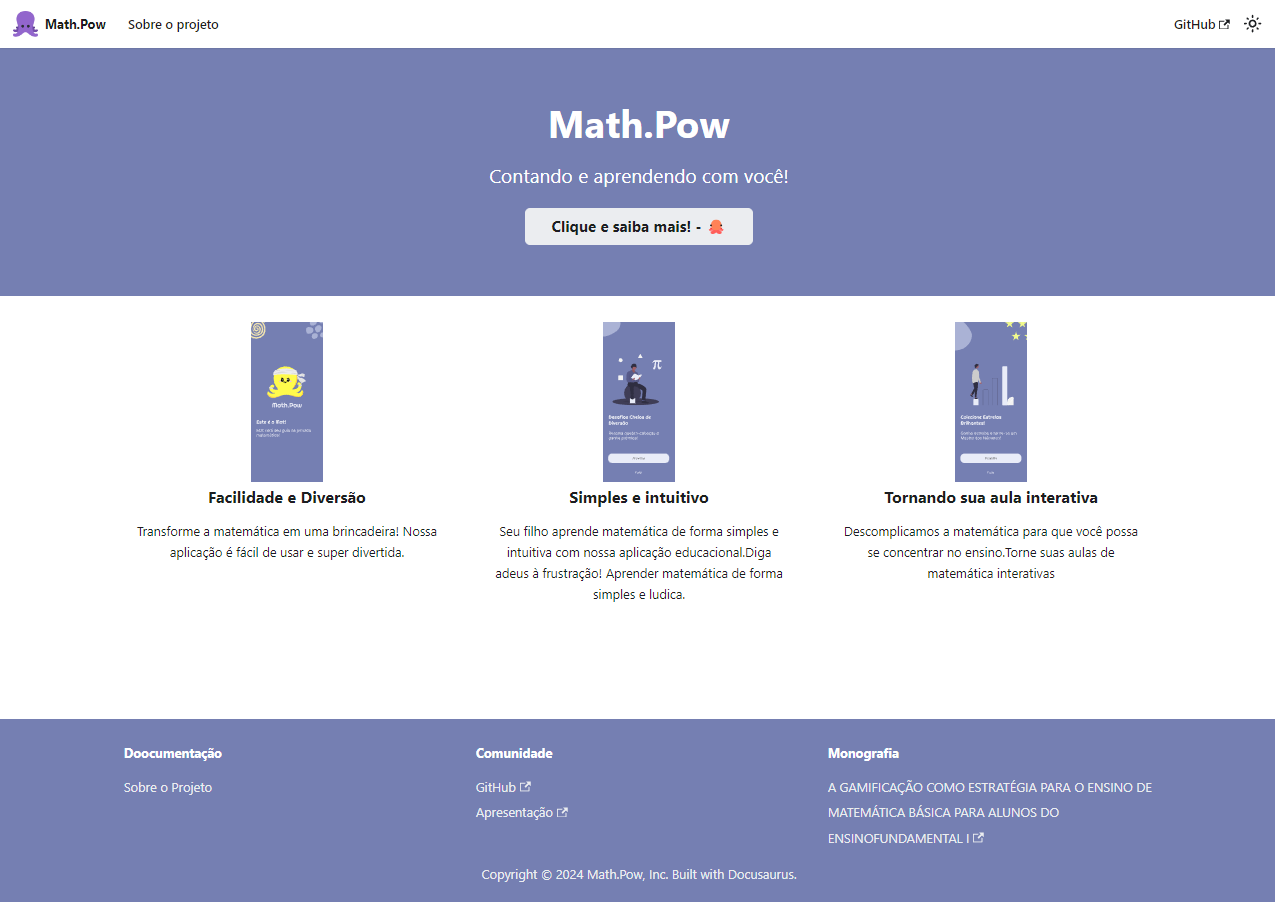
\includegraphics[width=0.8\linewidth]{figuras/Math.Pow App/mathPow.png}
    \caption{Imagem do site do projeto. Fonte: \url{https://mathpow.vercel.app/}}
    \label{fig:Figma}
\end{figure}

 
